\documentclass[10pt]{article}

%%%%%%%%%%%%%%%%%%%%%%%%%%%%%%%%%%%%%%%%%%%%%%%%%%%%%%%%%%%%%%%%%%%%%%%%%%%%%%%%
% LaTeX Imports
%%%%%%%%%%%%%%%%%%%%%%%%%%%%%%%%%%%%%%%%%%%%%%%%%%%%%%%%%%%%%%%%%%%%%%%%%%%%%%%%
\usepackage{amsfonts}                                                   % Math fonts
\usepackage{amsmath}                                                    % Math formatting
\usepackage{amssymb}                                                    % Math formatting
\usepackage{amsthm}                                                     % Math Theorems
\usepackage{arydshln}                                                   % Dashed hlines
\usepackage{attachfile}                                                 % AttachFiles
\usepackage{cancel}                                                     % Cancelled math
\usepackage{caption}                                                    % Figure captioning
\usepackage{color}                                                      % Nice Colors
\input{./lib/dragon.inp}                                                % Tikz dragon curve
\usepackage[ampersand]{easylist}                                        % Easy lists
\usepackage{fancyhdr}                                                   % Fancy Header
\usepackage[T1]{fontenc}                                                % Specific font-encoding
%\usepackage[margin=1in, marginparwidth=2cm, marginparsep=2cm]{geometry} % Margins
\usepackage{graphicx}                                                   % Include images
\usepackage{hyperref}                                                   % Referencing
\usepackage[none]{hyphenat}                                             % Don't allow hyphenation
\usepackage{lipsum}                                                     % Lorem Ipsum Dummy Text
\usepackage{listings}                                                   % Code display
\usepackage{marginnote}                                                 % Notes in the margin
\usepackage{microtype}                                                  % Niceness
\usepackage{lib/minted}                                                 % Code display
\usepackage{multirow}                                                   % Multirow tables
\usepackage{pdfpages}                                                   % Include pdfs
\usepackage{pgfplots}                                                   % Create Pictures
\usepackage{rotating}                                                   % Figure rotation
\usepackage{setspace}                                                   % Allow double spacing
\usepackage{subcaption}                                                 % Figure captioning
\usepackage{tikz}                                                       % Create Pictures
\usepackage{tocloft}                                                    % List of Equations
%%%%%%%%%%%%%%%%%%%%%%%%%%%%%%%%%%%%%%%%%%%%%%%%%%%%%%%%%%%%%%%%%%%%%%%%%%%%%%%%
% Package Setup
%%%%%%%%%%%%%%%%%%%%%%%%%%%%%%%%%%%%%%%%%%%%%%%%%%%%%%%%%%%%%%%%%%%%%%%%%%%%%%%%
\hypersetup{%                                                           % Setup linking
    colorlinks=true,
    linkcolor=black,
    citecolor=black,
    filecolor=black,
    urlcolor=black,
}
\RequirePackage[l2tabu, orthodox]{nag}                                  % Nag about bad syntax
\renewcommand*\thesection{\arabic{section} }                             % Reset numbering
\renewcommand{\theFancyVerbLine}{ {\arabic{FancyVerbLine} } }              % Needed for code display
\renewcommand{\footrulewidth}{0.4pt}                                    % Footer hline
\setcounter{secnumdepth}{3}                                             % Include subsubsections in numbering
\setcounter{tocdepth}{3}                                                % Include subsubsections in toc
%%%%%%%%%%%%%%%%%%%%%%%%%%%%%%%%%%%%%%%%%%%%%%%%%%%%%%%%%%%%%%%%%%%%%%%%%%%%%%%%
% Custom commands
%%%%%%%%%%%%%%%%%%%%%%%%%%%%%%%%%%%%%%%%%%%%%%%%%%%%%%%%%%%%%%%%%%%%%%%%%%%%%%%%
\newcommand{\nvec}[1]{\left\langle #1 \right\rangle}                    %  Easy to use vector
\newcommand{\ma}[0]{\mathbf{A} }                                         %  Easy to use vector
\newcommand{\mb}[0]{\mathbf{B} }                                         %  Easy to use vector
\newcommand{\abs}[1]{\left\lvert #1 \right\rvert}                       %  Easy to use abs
\newcommand{\pren}[1]{\left( #1 \right)}                                %  Big parens
\let\oldvec\vec
\renewcommand{\vec}[1]{\oldvec{\mathbf{#1} } }                            %  Vector Styling
\newtheorem{thm}{Theorem}                                               %  Define the theorem name
\newtheorem{definition}{Definition}                                     %  Define the definition name
\definecolor{bg}{rgb}{0.95,0.95,0.95}
\newcommand{\java}[4]{\vspace{10pt}\inputminted[firstline=#2,
                                 lastline=#3,
                                 firstnumber=#2,
                                 gobble=#4,
                                 frame=single,
                                 label=#1,
                                 bgcolor=bg,
                                 linenos]{java}{#1} }
\newcommand{\python}[4]{\vspace{10pt}\inputminted[firstline=#2,
                                 lastline=#3,
                                 firstnumber=#2,
                                 gobble=#4,
                                 frame=single,
                                 label=#1,
                                 bgcolor=bg,
                                 linenos]{python}{#1} }
\newcommand{\js}[4]{\vspace{10pt}\inputminted[firstline=#2,
                                 lastline=#3,
                                 firstnumber=#2,
                                 gobble=#4,
                                 frame=single,
                                 label=#1,
                                 bgcolor=bg,
                                 linenos]{js}{#1} }
%%%%%%%%%%%%%%%%%%%%%%%%%%%%%%%%%%%%%%%%%%%%%%%%%%%%%%%%%%%%%%%%%%%%%%%%%%%%%%%%
% Beginning of document items - headers, title, toc, etc...
%%%%%%%%%%%%%%%%%%%%%%%%%%%%%%%%%%%%%%%%%%%%%%%%%%%%%%%%%%%%%%%%%%%%%%%%%%%%%%%%
\pagestyle{fancy}                                                       %  Establishes that the headers will be defined
\fancyhead[LE,LO]{Computer Systems Notes}                                  %  Adds header to left
\fancyhead[RE,RO]{Zoe Farmer}                                       %  Adds header to right
\cfoot{ \thepage }
\lfoot{CSCI 2400}
\rfoot{Han}
\title{Computer Systems Notes}
\author{Zoe Farmer}

%%%%%%%%%%%%%%%%%%%%%%%%%%%%%%%%%%%%%%%%%%%%%%%%%%%%%%%%%%%%%%%%%%%%%%%%%%%%%%%%
% Beginning of document items - headers, title, toc, etc...
%%%%%%%%%%%%%%%%%%%%%%%%%%%%%%%%%%%%%%%%%%%%%%%%%%%%%%%%%%%%%%%%%%%%%%%%%%%%%%%%
\pagestyle{fancy}                                                       %  Establishes that the headers will be defined
\fancyhead[LE,LO]{Homework 2}                                  %  Adds header to left
\fancyhead[RE,RO]{Zoe Farmer}                                       %  Adds header to right
\cfoot{\mlptikz[size=0.25in, text=on, textposx=0, textposy=0, textvalue=\thepage, textscale=0.75in]{applejack}}
\lfoot{APPM 3570}
\rfoot{Kleiber}
\title{Homework 2}
\date{Kleiber}
\author{Zoe Farmer - 101446930}
%%%%%%%%%%%%%%%%%%%%%%%%%%%%%%%%%%%%%%%%%%%%%%%%%%%%%%%%%%%%%%%%%%%%%%%%%%%%%%%%
% Beginning of document items - headers, title, toc, etc...
%%%%%%%%%%%%%%%%%%%%%%%%%%%%%%%%%%%%%%%%%%%%%%%%%%%%%%%%%%%%%%%%%%%%%%%%%%%%%%%%
\begin{document}

\maketitle

\begin{easylist}[enumerate]
    @ Chapter 1, p. 17: \#32
    @@ An elevator starts at the basement with 8 people (not including the elevator operator) and discharges them all by the time it reaches the top floor, number 6. In how many ways could the operator have perceived the people leaving the elevator if all people look alike to him? What if the 8 people consisted of 5 men and 3 women and the operator could tell a man from a woman?
    @@@ In the first part of this problem we can view the 8 individuals as indistinguishable balls, and the floors as distinguishable urns. Therefore, we can rephrase the problem to look as such:

    \[ \underbrace{x_1 + x_2 + x_3 + x_4 + x_5 + x_6}_{Urns} = \underbrace{8}_{Balls} \]

    If we also allow for no individuals to leave on certain floors, there are a known amount of solutions.

    \[ \begin{pmatrix}n + r - 1\\ r - 1\end{pmatrix} \Rightarrow \boxed{\begin{pmatrix}13\\5\end{pmatrix}} \]

    @@@ For the second part of the problem, if the idiot operator can now discern the difference between a man and a woman, the problem is phrased in two parts.

    \[ \begin{cases}
            x_1 + x_2 + x_3 + x_4 + x_5 + x_6 = 5 \Rightarrow \begin{pmatrix}10\\5\end{pmatrix}\\\\
            x_1 + x_2 + x_3 + x_4 + x_5 + x_6 = 3 \Rightarrow \begin{pmatrix}8\\5\end{pmatrix}\\
    \end{cases} \]

    However this only accounts for the two separate groups. In order to obtain the total number of solutions, they must be multiplied together. So the final answer is

    \[ \boxed{\begin{pmatrix}10\\5\end{pmatrix} \cdot \begin{pmatrix}8\\5\end{pmatrix}} \]

    @ Chapter 2, p. 48: \#2, 4, 8, 9; p. 52 \#6, 7.
    @@ In an experiment, die is rolled continually until a 6 appears, at which point the experiment stops. What is the sample space of this experiment? Let $E_n$ denote the event that $n$ rolls are necessary to complete the experiment. What points of the sample space are contained in $E_n$? What is ${\left( \bigcup^\infty_1 E_n \right)}^c$?
    @@@ Assuming the die in question is a six-sided die, The sample space for this experiment is

       \[ \left\{ (6), (1,6), (2, 6), (3, 6), \cdots, (1, 1, 6), (1, 2, 6), \cdots \right\} \]

       If the die is not a D6, this pattern holds true for numbers greater than six, since rolling six is our only end condition.

    @@@ In any event, $E_n$, the die may roll any number in the sample space, therefore $E_n$ covers all points in the sample space.
    @@@ Going off our previous statement, since any event is possible, the complement of the union equals the null set.

       \[{\left( \bigcup^\infty_1 E_n \right)}^c = \emptyset \]

    @@ $A$, $B$, and $C$ take turns flipping a coin. The first one to get a head wins. The sample space of this experiment can be defined by
       \[ S = \left\{ 1, 01, 001, 0001, \cdots, 000000\cdots \right\} \]
    @@@ Interpret the sample space.
    @@@@ Since there are only two outcomes for each toss, the game will continue until a player flips heads. Therefore the space is infinite in cardinality, and all events end with a heads.
    @@@ Define the following events in terms of $S$:
    @@@@ $A$ wins $ = A \to $ This creates a new set, one where $A$ is the winner.
       \[ E_A = \left\{ x | x \in S \wedge 1_i \equiv 1 \mod 3 \right\} \text{ and } E_A \subset S \]
       Where $1_i$ is the index of the heads.
    @@@@ $B$ wins $ = B \to$ Again, a new event set is created, however this time with $B$ the winner.
       \[ E_B = \left\{ x | x \in S \wedge 1_i \equiv 2 \mod 3 \right\} \text{ and } E_B \subset S \]
       Where $1_i$ is the index of the heads.
    @@@@ ${(A \cup B)}^c \to$ This is the same as asking for every event where $C$ is the winner.
       \[ E_C = \left\{ x | x \in S \wedge 1_i \equiv 3 \mod 3 \right\} \text{ and } E_C \subset S \]
       Where $1_i$ is the index of the heads.

    @@ Suppose that $A$ and $B$ are mutually exclusive events for which $P(A) = .3$ and $P(B) = .5$. What is the probability that
    @@@ either $A$ or $B$ occurs?
    @@@@ Since they are mutually exclusive, this can be expressed as $P(A) + P(B) = \boxed{0.8}$.
    @@@ $A$ occurs but $B$ does not?
    @@@@ Again, they are mutually exclusive, so if $A$ occurs, $B$ by definition will not. Therefore we just need the probability of $A \to P(A) = 0.3$
    @@@ both $A$ and $B$ occur?
    @@@@ By definition of mutually exclusive, the events cannot both occur. Therefore the probability of this event is zero.

    @@ A retail establishment accepts either the American Express or the VISA credit card. A total of 24 percent of its customers carry an American Express card, 61 percent carry a VISA card, and 11 percent carry both cards. What percentage of its customers carry a credit card that the establishment will accept?
    @@@ This can be solved with the exclusion/inclusion principle. Let $A$ be the set of American Express cardholders, $B$ be the set of VISA cardholders, and $C$ be those that carry both.
        \[ |A| + |B| - |C| \to 24 + 61 - 11 = 74 \]
       Therefore $74$\% of the customers carry a valid card.

    @@ Let $E$, $F$, and $G$ be three events. Find expressions for the events so that, of $E$, $F$, and $G$,
    @@@ only $E$ occurs: $E \cap F^c \cap G^c$
    @@@ both $E$ and $G$, but not $F$, occur: $(E \cap G) \cap F^c$
    @@@ at least one of the events occurs: $E \cup F \cup G$
    @@@ at least two of the events occur: $((E \cap F) \cap G^c) \cup ((E \cap G) \cap F^c) \cup ((F \cap G) \cap E^c) \cup (E \cap F \cap G)$
    @@@ all three events occur: $ E \cap F \cap G$
    @@@ none of the events occurs: $ {(E \cup F \cup G)}^c$
    @@@ at most one of the events occurs: $(E \cap F^c \cap G^c) \cup (F \cap G^c \cap E^c) \cup (G \cap E^c \cap F^c)$
    @@@ at most two of the events occur: ${(E \cap F \cap G)}^c$
    @@@ exactly two of the events occur: $((E \cap F) \cap G^c) \cup ((E \cap G) \cap F^c) \cup ((F \cap G) \cap E^c)$
    @@@ at most three of the events occur: since we only have three events, this is the entire sample space.

    @@ Find the simplest expression for the following
    events:
    @@@ $(E \cup F)(E \cup F^c) \to (F \cap F^c) \cup E \to E$
    @@@ $(E \cup F)(E^c \cup F)(E \cup F^c) \to (E \cap E^c \cup F)(E \cup F^c) \to E \cap F$
    @@@ $(E \cup F)(F \cup G) \to (E \cap G) \cup F$

    @ True or False: If true, prove the statement is true. If false, explain why or give a counterexample.
    @@ $(E \cup F)(E \cup F^c)$ is the empty set. This statement is false. This results in $E$ since $F \cup F^c \to S$ and $S \cap E \to E$.
    @@ $F = FE \cup FE^c \to $ True. This is also shown as $ ( E \cup E^c ) F \to S \cap F \to F$.
    @@ $P(EF^c) = P(E) - P(EF) \to $ True. The first statement is asking for all events that occur where event $E$ and the complement of $F$ intersect. This is limited to all events in $E$ that aren't also in $F$, which is exactly what the second part asks for.
    @@ $P(\text{exactly one of the events $E$ or $F$ occurs but not both}) = P(E) + P(F ) - 2P(EF) \to$ True. This is asking for the probabilities of both events occurring, but not at the same time. In other words, the probability of $E$ minus $EF$ as well as the probability of $F$ minus $EF$. This results in the right hand side of the equation.

    @ Suppose a city has three newspapers: $a$, $b$, and $c$. Let $A$ represent the event that the person reads newspaper $a$, $B$ the event that the person reads $b$, and similarly for event $C$. A randomly chosen person reads 0, 1, 2, or all 3 newspapers.
    @@ List all elements in the sample space. Clearly explain your notation.
    @@@ Any randomly chosen individual can read 0, 1, 2, or 3 newspapers. Therefore, for any individual $M$, the sample space of their newspaper readings can be expressed as

    \[ S = \left\{
                \underbrace{()}_{\text{0 Read}},
                \underbrace{(a), (b), (c)}_{\text{1 Read}},
                \underbrace{(ab), (ac), (bc)}_{\text{2 Read}},
                \underbrace{(abc)}_{\text{3 Read}}
        \right\} \]

    @@ Suppose events $A$, $B$ and $C$ have the following probabilities: $P(A) = 0.30, P(B) = 0.35, P(C) = 0.40, P(A \cap B) = 0.06, P(A \cap C) = 0.11, P(B \cap C) = 0.16$ and $P(A \cap B \cap C) = 0.01$. For each of the following events, describe it with a Venn diagram, describe it with set notation (using your sample space from part (a)), and find its probability.
    @@@ The event that a randomly chosen person reads only one newspaper.
    @@@@ This event can be described as the union of the three sets, minus any overlap. Using our sample space from before, we can look at this as all events with the individual reading one newspaper.

        \[ E = \left\{ (a), (b), (c) \right\} \]

        We can create a Venn diagram in order to fully understand what's going on.

        \begin{figure}[!ht]
            \centering
            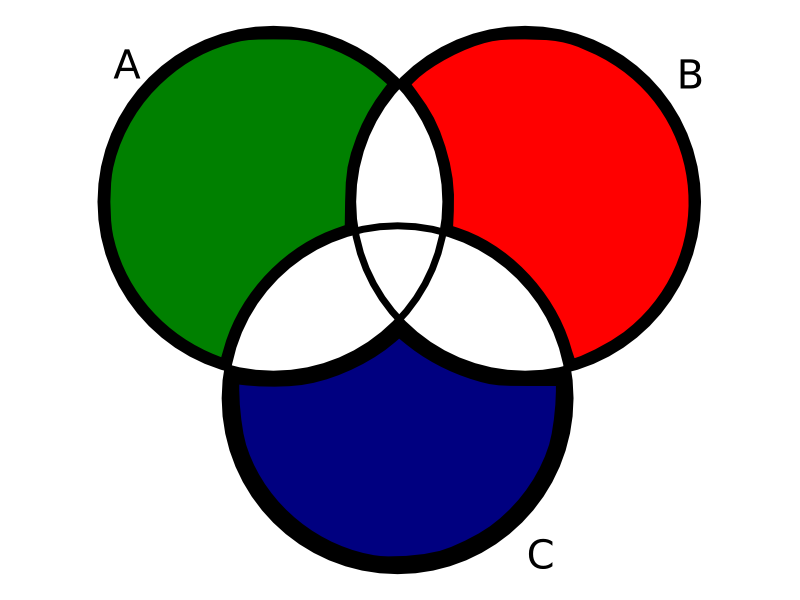
\includegraphics[scale=0.25]{./img/venn1.png}
        \end{figure}

        And the probability of this event will be

        \[ P(A) + P(B) + P(C) - 2 P(A \cap B) - 2 P(A \cap C) - 2 P(B \cap C) + 3 P(A \cap B \cap C) \]

        Inputting numeric values for these probabilities yields

        \[ 1.05 - 0.12 - 0.22 - 0.32 + 0.03 = \boxed{0.42} \]

    @@@ The event that a randomly selected person reads at least two newspapers.
    @@@@ This event can be described as the intersections of all three sets. Using our previous sample space again, we can describe this as two or more newspapers.

        \[ E = \left\{ (ab), (ac), (bc), (abc) \right\} \]

        We can create a Venn diagram in order to fully understand what's going on.

        \begin{figure}[!ht]
            \centering
            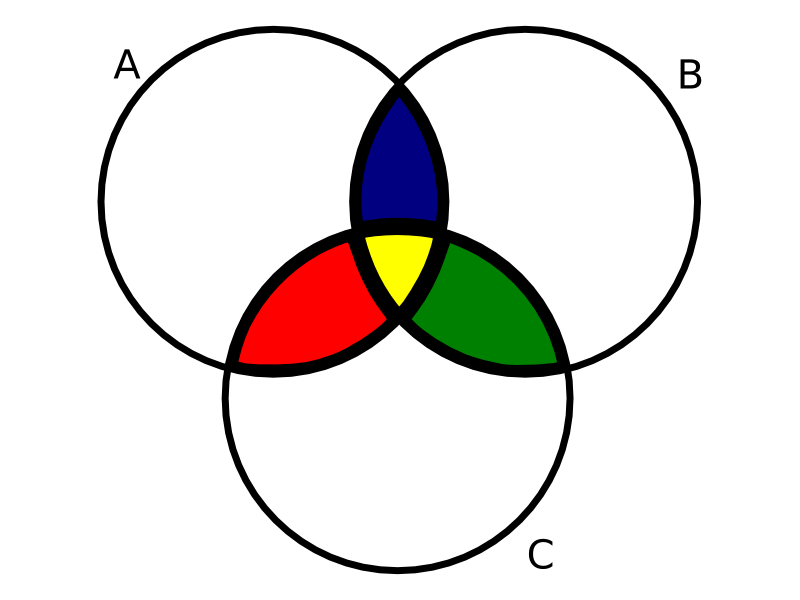
\includegraphics[scale=0.25]{./img/venn2.png}
        \end{figure}

        And the probability of this event will be

        \[ P(A \cap B) + P(A \cap C) + P(B \cap C) - 3 P(A \cap B \cap C) \]

        Inputting numeric values yields

        \[ 0.06 + 0.11 + 0.16 - 0.03 = \boxed{0.30} \]

    @@@ The event that a randomly selected person does not read any of the newspapers.
    @@@@ This event is the sample space minus the unions of all three sets. Using our sample space this is described as the sample space without the events.

        \[ \left\{ () \right\} \]

        We can create a Venn diagram for this event.

        \begin{figure}[!ht]
            \centering
            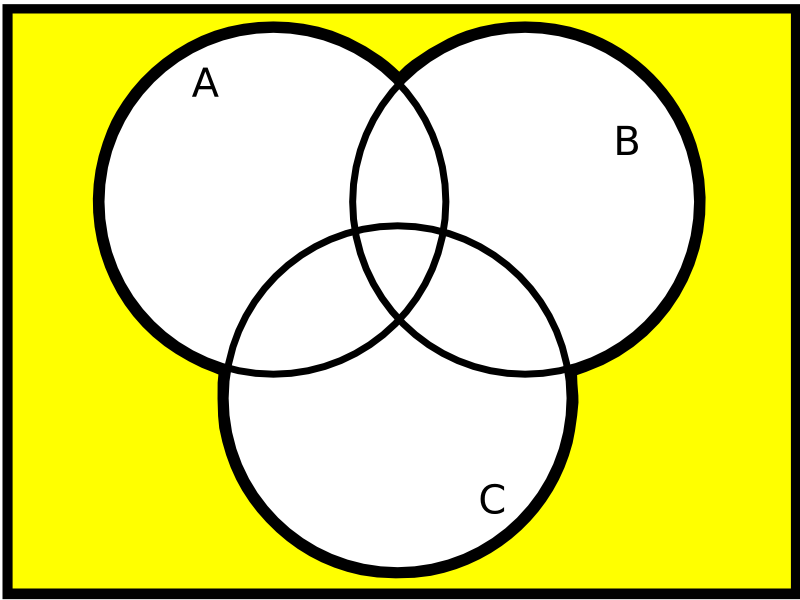
\includegraphics[scale=0.25]{./img/venn3.png}
        \end{figure}

        And the probability will be

        \[ 1 - \left( P(A) + P(B) + P(C) - P(A \cap B) - P(A \cap C) - P(B \cap C) + P(A \cap B \cap C) \right) \]

        Inputting numeric values yields

        \[ 1 - (0.3 + 0.35 + 0.4 - 0.06 - 0.11 - 0.16 + 0.01) = \boxed{0.27} \]

    @@@ The event that the person reads newspaper $a$, but not $b$ or $c$.
    @@@@ This event is just event $A$, with no other set intersections. Using our sample space this is shown as

        \[ \left\{ (a) \right\} \]

        We can create a Venn diagram for this event.

        \begin{figure}[!ht]
            \centering
            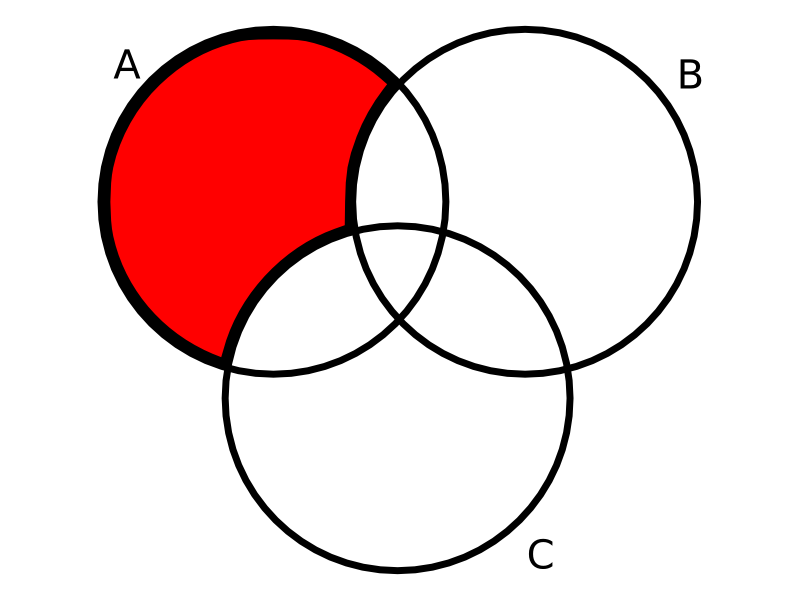
\includegraphics[scale=0.25]{./img/venn4.png}
        \end{figure}

        And the probability will be

        \[ P(A) - P(A \cap B) - P(A \cap C) + P(A \cap B \cap C) \]

        Inputting numeric values yields

        \[ 0.30 - 0.06 - 0.11 + 0.01 = \boxed{0.13} \]

    @ Suppose there are 15 people in a room, 8 men and 7 women. Five people will be selected to serve on a committee. Suppose every combination has equal probability.
    @@ What is the sample space, $S$ (describe in words or in symbols), and its cardinality, $|S|$?
    @@@ The sample space, $S$, is all combinations of people selected. If we let $R$ represent the room of people to choose from

        \[ S = \left\{ (x_1, x_2, x_3, x_4, x_5) | x_n \in R, x_n \text{ is unique}, \text{ no combination is repeated} \right\} \]

    It's cardinality therefore can be expressed as

        \[ |S| = \begin{pmatrix}15\\5\end{pmatrix} \Rightarrow \frac{15!}{5!10!} \Rightarrow 3003 \]

    @@ Let $A$ be the event that 3 men and 2 women are selected. What is the probability of $A$?
    @@@ In order to solve this we need to determine how many combinations there are with 3 men and 2 women. This can be broken up into two separate parts.

        \[ \begin{pmatrix}8\\3\end{pmatrix} \cdot \begin{pmatrix}7\\2\end{pmatrix} \Rightarrow 1176 \]

        According to our previous result, the cardinality of the set is 3003, meaning each combination has a 1 in 3003 chance of occurring. Therefore, this probability is merely

        \[ \frac{1}{\begin{pmatrix}15\\5\end{pmatrix}} \cdot \begin{pmatrix}8\\3\end{pmatrix} \cdot \begin{pmatrix}7\\2\end{pmatrix} = \boxed{\frac{56}{143} \approx 0.3916} \]

    @@ Let $B$ be the event that at least 2 women serve on the committee. What is the probability of $B$?
    @@@ Again the key to this problem is to identify how many combinations satisfy the condition, and then determine the probability based off the cardinality. Since all conditions are mutually exclusive, we can look at them independently.

    \[
        \frac{1}{\begin{pmatrix}15\\5\end{pmatrix}} \cdot
            \left( \begin{pmatrix}7\\2\end{pmatrix}\begin{pmatrix}8\\3\end{pmatrix} +
            \begin{pmatrix}7\\3\end{pmatrix}\begin{pmatrix}8\\2\end{pmatrix} +
            \begin{pmatrix}7\\4\end{pmatrix}\begin{pmatrix}8\\1\end{pmatrix} +
            \begin{pmatrix}7\\5\end{pmatrix}\begin{pmatrix}8\\0\end{pmatrix} \right) =
        \boxed{\frac{9}{11} \approx 0.818182}
    \]

    @@ What is the event $A \cap B$ (describe in words or in symbols)? What is its probability?
    @@@ This event is when there are at least two women, intersected with two women and three men. This results in a committee where there are two women and three men. The probability of this event is the same as it is above, namely

        \[ \frac{1}{\begin{pmatrix}15\\5\end{pmatrix}} \cdot \begin{pmatrix}8\\3\end{pmatrix} \cdot \begin{pmatrix}7\\2\end{pmatrix} = \boxed{\frac{56}{143} \approx 0.3916} \]

    @@ Suppose one man and one woman are married and, by the rules of the committee, can not serve together. How does the sample space change in this situation? Re-calculate $P(A)$ and $P(B)$.
    @@@ In this situation the sample space shifts to only include committees without the couple together, however they can serve independently. Let $y_1$ and $y_2$ be our couple. Therefore, the sample space now becomes

    \[
        \begin{aligned}
             S = \{ (x_1, x_2, x_3, x_4, x_5) | & x_n \in R,\\
                                                     & x_n \text{ is unique},\\
                                                     & \text{no combination is repeated},\\
                                                     & y_1, y_2 \text{ not in the set together} \}
        \end{aligned}
    \]

    $P(A)$ adjusts accordingly.

    \[
        \frac{1}{\begin{pmatrix}15\\5\end{pmatrix}}
        \left(
            \begin{pmatrix}7\\3\end{pmatrix} \begin{pmatrix}6\\2\end{pmatrix} \begin{pmatrix}2\\1\end{pmatrix}
        \right) = \boxed{\frac{50}{143} \approx 0.34965}
    \]

    As does $P(B)$.

    \[
        \frac{1}{\begin{pmatrix}15\\5\end{pmatrix}} \cdot
        \left(
            \begin{pmatrix}6\\2\end{pmatrix}\begin{pmatrix}7\\3\end{pmatrix}\begin{pmatrix}2\\1\end{pmatrix}+
            \begin{pmatrix}6\\3\end{pmatrix}\begin{pmatrix}7\\2\end{pmatrix}\begin{pmatrix}2\\1\end{pmatrix}+
            \begin{pmatrix}6\\4\end{pmatrix}\begin{pmatrix}7\\1\end{pmatrix}\begin{pmatrix}2\\1\end{pmatrix}+
            \begin{pmatrix}7\\5\end{pmatrix}\begin{pmatrix}8\\0\end{pmatrix} \right) =
        \boxed{\frac{101}{143} \approx 0.706294}
    \]

\end{easylist}

\end{document}
